\documentclass[12pt]{article}
\usepackage{amssymb}
\usepackage{amsmath}
\usepackage{mathtools}
\usepackage[utf8]{inputenc}
\usepackage{hyperref}
\usepackage{comment}
\usepackage{polski}
\usepackage{mathrsfs}
\usepackage{geometry}
\usepackage{amsthm}
\usepackage{csquotes}
\usepackage{float}
\geometry{a4paper, portrait, margin=1in}


\usepackage[breaklinks=true]{hyperref}

\setlength\parindent{0pt}

\DeclarePairedDelimiter\abs{\lvert}{\rvert}%
\DeclarePairedDelimiter\norm{\lVert}{\rVert}%

% Swap the definition of \abs* and \norm*, so that \abs
% and \norm resizes the size of the brackets, and the 
% starred version does not.
\makeatletter
\let\oldabs\abs
\def\abs{\@ifstar{\oldabs}{\oldabs*}}
%
\let\oldnorm\norm
\def\norm{\@ifstar{\oldnorm}{\oldnorm*}}
\makeatother

\newcommand{\Cov}{\mathrm{Cov}}
\newcommand{\corr}{\mathrm{corr}}
\newcommand{\pH}{\mathscr{H}}
\newcommand{\bH}{\mathscr{B}(\mathscr{H})}
\newcommand{\gH}{\mathscr{G}(\mathscr{H})}
\newcommand{\complex}{\mathbb{C}}
\newcommand{\real}{\mathbb{R}}
\newcommand*\conj[1]{\overline{#1}}
\newcommand*\dotprod[2]{\langle #1 , #2 \rangle}
\newtheorem{theorem}{Twierdzenie}[section]
\newtheorem{corollary}{Wniosek}[theorem]
\newtheorem{lemma}[theorem]{Lemat}
\newtheorem{fact}[theorem]{Fakt}
\newtheorem{definition}[theorem]{Def.}
\newtheorem{example}[theorem]{Pd.}
\newcommand{\pder}[2][]{\frac{\partial#1}{\partial#2}}
% Command for partial derivatives. The first argument denotes the function and the second argument denotes the variable with respect to which the derivative is taken. The optional argument denotes the order of differentiation. The style (text style/display style) is determined automatically
\providecommand{\pd}[3][]{\ensuremath{
\ifinner
\tfrac{\partial{^{#1}}#2}{\partial{#3^{#1}}}
\else
\dfrac{\partial{^{#1}}#2}{\partial{#3^{#1}}}
\fi
}}



\title{Projekt III - Quanto.}
\author{Wojciech Fica \footnote{\href{mailto:wojtekfica@gmail.com}{wojtekfica@gmail.com}}, Dominik Jaźwiecki \footnote{\href{mailto:dominik.jazwiecki@o2.pl}{dominik.jazwiecki@o2.pl}}, Krzysztof Kowalski \footnote{\href{mailto:KKowalski351@gmail.com}{KKowalski351@gmail.com}}}
\date{\today}

\begin{document}

\maketitle
%\tableofcontents
%\pagebreak

\section{Wstęp}
\label{Opcja quanto}

W projekcie przeanalizujemy zachowanie opcji typu quanto. Zakładamy, że aktywem bazowym będzie złoto notowane w USD (London Gold Fixing Price). Przyjmujemy, że
zarówno ceny złota, jak i kurs wymiany USDPLN są modelowane przez skorelowane geometryczne ruchy
Browna.

Rozważamy instrument wypłacający w chwili $T$ = 2020-06-30 wartość 
$$ 100 \text{PLN} * \max \left(\frac{S(T)}{S(0)} - K, 0 \right),$$ 
gdzie $0 \leq K \leq 2$, chwila 0 to 2019-06-30, a $S(t)$ to cena złota w chwili $t$ w dolarach.

\section{Wycena instrumentu typu Quanto.}
\subsection{Wycena uwzględniająca kurs wymiany walut i cenę złota w dolarach.}
\label{Wariant 1}

Przyjmujemy, że zarówno cena złota wyrażona w dolarach, $S(t)$ , jak i kurs wymiany USDPLN - ile złotych to jeden dolar, $S_\$(t)$, są modelowane przez skorelowane geometryczne ruchy Browna.
\begin{align*}
dS &= \mu S dt + \sigma S dX_1 \\
dS_\$ &= \mu_\$ S_\$ dt + \sigma_\$ S_\$ dX_2,
\end{align*}
gdzie 
$$
    \corr(X_1, X_2) = \rho.
$$
Konstruujemy portfel zabezpieczający powyższą opcję. 
\begin{align*}
\Pi = V(S_\$, S, t) - \Delta_\$ S_\$ - \Delta S S_\$    
\end{align*}
W powyższym wzorze wszystkie wartości są wyrażone w PLN. 
\begin{enumerate}
    \item $\Delta_\$ $ to liczba dolarów w pozycji krótkiej,
    \item $\Delta$ to ilość aktywa podstawowego, złota, w pozycji krótkiej.
\end{enumerate}
Korzystając z dwuwymiarowego wzoru Ito otrzymujemy:
\begin{align*}
    d\Pi =  &\left( \pd{V}{t} + \tfrac{1}{2} \sigma_\$^2 S_\$^2 \pd[2]{V}{S_\$}  + \rho \sigma_\$ \sigma S_\$ S \tfrac{\partial^2 V}{\partial S_\$\partial S} + \tfrac{1}{2} \sigma^2 S^2 \pd[2]{V}{S} - \rho \sigma_\$ \sigma \Delta S_\$ S - r_f \Delta_\$ S_\$ \right) dt + \\
            &\left( \pd{V}{S_\$} - \Delta_\$ - \Delta S \right) dS_\$ + \\
            &\left( \pd{V}{S} - \Delta S_\$ \right) dS, 
\end{align*}
gdzie $r_f$ stopa nie obciążona ryzykiem w USD.
Dobierając 

\begin{align*}
    \Delta_\$ = \pd{V}{S_\$} - \tfrac{S}{S_\$} \pd{V}{S} \\
    \Delta = \tfrac{1}{S_\$} \pd{V}{S}
\end{align*}
eliminujemy ryzyko. Zatem zwroty z portfela $\Pi$ są takie same jak zwroty z obligacji nie obciążonej ryzykiem w PLN - $r$:
\begin{align*}
    \left( \pd{V}{t} + \tfrac{1}{2} \sigma_\$^2 S_\$^2 \pd[2]{V}{S_\$}  + \rho \sigma_\$ \sigma S_\$ S \tfrac{\partial^2 V}{\partial S_\$\partial S} + \tfrac{1}{2} \sigma^2 S^2 \pd[2]{V}{S} - \rho \sigma_\$ \sigma \Delta S_\$ S - r_f \Delta_\$ S_\$ \right) dt = r \Pi dt,
\end{align*}
czyli 
\begin{align*}
    \pd{V}{t} + \tfrac{1}{2} \sigma_\$^2 S_\$^2 \pd[2]{V}{S_\$}  + \rho \sigma_\$ \sigma S_\$ S \tfrac{\partial^2 V}{\partial S_\$\partial S} + \tfrac{1}{2} \sigma^2 S^2 \pd[2]{V}{S} - \rho \sigma_\$ \sigma \Delta S_\$ S  - r_f \Delta_\$ S_\$ = r (V- \Delta_\$ S_\$ - \Delta S S_\$).
\end{align*}
Podstawiamy wyliczone wcześniej delty i otrzymujemy równanie różniczkowe opisujące cenę rozważanej opcji. 
\begin{align}\label{eqn:1}
    \pd{V}{t} + \tfrac{1}{2} \sigma_\$^2 S_\$^2 \pd[2]{V}{S_\$}  + \rho \sigma_\$ \sigma S_\$ S \tfrac{\partial^2 V}{\partial S_\$\partial S} + \tfrac{1}{2} \sigma^2 S^2 \pd[2]{V}{S} + (r- r_f) S_\$ \pd{V}{S_\$} + (r_f - \rho \sigma_\$ \sigma) S \pd{V}{S} - rV = 0.
\end{align}

Przypomnijmy warunek brzegowy dla tego równania:
\begin{align*}
    V(S_\$, S, T) =  100 \text{PLN} * \max \left(\tfrac{S(T)}{S(0)} - K, 0 \right) = \tfrac{100}{S(0)} \max( S(T) - KS(0), 0)
\end{align*}
Poczyńmy dwie ważne obserwacje:
\begin{enumerate}
    \item Warunek brzegowy mówi, że opcja wypłaca tyle samo co $\tfrac{100}{S(0)}$ opcji call z ceną wykonania $KS(0), $ a przecież w chwili $t=0$ znamy $S(0)$ i $K$. 
    \item Warunek brzegowy nie zależy od $S_\$$ więc możemy spróbować poszukać rozwiązania równania \ref{eqn:1}, które zależy tylko od $S$ i $t$. 
\end{enumerate}
 Szukamy $W(S, t)$, że 
 $$
    V(S_\$, S, t) = W(S, t).
 $$
 Wtedy równanie \ref{eqn:1} upraszcza się do 
 \begin{align*}
     \pd{W}{t} + \tfrac{1}{2} \sigma^2 S^2 \pd[2]{W}{S} + (r - (r - r_f +\rho \sigma_\$ \sigma )) S \pd{W}{S} - rW = 0.
 \end{align*}
 Co jest klasycznym równaniem Black-Scholes'a z dywidendą $D = r - r_f + \rho \sigma_\$ \sigma$, na które są znane jawne wzory. 
 \newline

 Podsumowując, opcja powyższa opcja quanto jest warta tyle samo co $\tfrac{100}{S(0)}$ opcji call z ceną wykonania $KS(0)$ na aktywo bazowe wypłacające wypłacające ciągłą dywidendę $D = r - r_f +\rho \sigma_\$ \sigma$.  
 \newline
 
 Zauważmy, że znamy wzory jawne na $W(s, t)$ oraz na $\pd{W}{S}$ - możemy zatem przeprowadzić symulację delta-hedgingu aby sprawdzić jak te teoretyczne rozważania wypadają w praktyce, co opiszemy w kolejnych sekcjach.
 

\subsection{Wycena uwzględniająca kurs wymiany walut i cenę złota w złotówkach.}
\label{Wariant 2}

Teraz przeprowadzimy podobną analizę jak w poprzednim paragrafie, ale tym razem posłużymy się procesem USDPLN oraz procesem wartości złota denominowanym w PLN. Przyjmiemy oznaczenia:
\begin{enumerate}
    \item $X_t$ - kurs wymiany USDPLN.
    \item $Y_t$ - wartość złota denominowana w PLN.
\end{enumerate}
Tak jak poprzednio zakładamy, że procesy są modelowane przez skorelowane geometryczne ruchy Browna.
\begin{align*}
dX &= \mu_1 X dt + \sigma_1 X dB_1 \\
dY &= \mu_2 Y dt + \sigma_2 Y dB_2,
\end{align*}
gdzie 
$$
    \corr(B_1, B_2) = \rho.
$$
Parametry procesów opiszemy w kolejnej sekcji gdzie omawiamy kalibrację modelu.
\newline
Konstruujemy portfel zabezpieczający powyższą opcję. 
\begin{align*}
\Pi = V(X, Y, t) - \Delta_1 X - \Delta_2 Y    
\end{align*}
W powyższym wzorze wszystkie wartości są wyrażone w PLN. 
\begin{enumerate}
    \item $\Delta_1 $ to liczba dolarów w pozycji krótkiej,
    \item $\Delta_2 $ to ilość aktywa podstawowego, złota, w pozycji krótkiej.
\end{enumerate}
Korzystając z dwuwymiarowego wzoru Ito otrzymujemy:
\begin{align*}
    d\Pi =  &\left( \pd{V}{t} + \tfrac{1}{2} \sigma_1^2 X^2 \pd[2]{V}{X}  + \rho \sigma_1 \sigma_2 X Y \tfrac{\partial^2 V}{\partial X\partial Y} + \tfrac{1}{2} \sigma_2^2 Y^2 \pd[2]{V}{Y} - r_f \Delta_1 X \right) dt + \\
            &\left( \pd{V}{X} - \Delta_1 \right) dX + \\
            &\left( \pd{V}{Y} - \Delta_2 \right) dY.
\end{align*}

Dobierając 
\begin{align*}
    \Delta_1 = \pd{V}{X} \hspace{1cm}    \Delta_2 = \pd{V}{Y}
\end{align*}
eliminujemy ryzyko. Zatem zwroty z portfela $\Pi$ są takie same jak zwroty z obligacji nie obciążonej ryzykiem w PLN, stopa $r$:
\begin{align*}
   \left( \pd{V}{t} + \tfrac{1}{2} \sigma_1^2 X^2 \pd[2]{V}{X}  + \rho \sigma_1 \sigma_2 X Y \tfrac{\partial^2 V}{\partial X\partial Y} + \tfrac{1}{2} \sigma_2^2 Y^2 \pd[2]{V}{Y} - r_f \Delta_1 X \right) dt = r \Pi dt,
\end{align*}
czyli 
\begin{align}\label{eq:2}
    \pd{V}{t} + \tfrac{1}{2} \sigma_1^2 X^2 \pd[2]{V}{X}  + \rho \sigma_1 \sigma_2 X Y \tfrac{\partial^2 V}{\partial X\partial Y} + \tfrac{1}{2} \sigma_2^2 Y^2 \pd[2]{V}{Y} - r_f \Delta_1 X = r (V - \pd{V}{X}X - \pd{V}{Y}Y)
\end{align}

Przypomnijmy warunek brzegowy dla tego równania:
\begin{align*}
    V(X, Y, T) =  100 \text{PLN} * \max \left(\tfrac{Y_TX_0}{X_TY_0} - K, 0 \right) = \tfrac{100 X_0}{Y_0} \max( Z_T - K\tfrac{Y_0}{X_0}, 0),
\end{align*}
gdzie 
\begin{align*}
    Z_t = \tfrac{Y_t}{X_t}.
\end{align*}
Skoro aby określić payoff wystarczy znać wartość procesu $Z_t$ (i jakieś stałe), to być może da się wycenić opcję używając tylko procesu $Z_t$. Szukamy takiego $W(Z, t)$, że
\begin{align*}
    V(X, Y, t) = W(Z, t), 
\end{align*}
gdzie $Z = \tfrac{Y}{X}$. Teraz, korzystając z reguły łańcucha, policzymy pochodne występujące we wzorze \ref{eq:2} i spróbujemy przepisać ten wzór tak, aby zależał on tylko od $Z$ i $t$.
Na przykład, 
\begin{align*}
    \pd{V}{t} = \pd{W}{t}
\end{align*}
oraz, stosując regułę łańcucha
\begin{align*}
    \pd{V}{X} = \pd{W}{Z} \pd{Z}{X} = - \pd{W}{Z} \tfrac{Y}{X^2}.
\end{align*}
Czyli czynnik $r \pd{V}{X}X  $ w równaniu [\ref{eq:2}] możemy zastąpić przez $- \pd{W}{Z}Z$. Rzeczywiście
\begin{align*}
    r \pd{V}{X}X = -r \pd{W}{Z} \tfrac{Y}{X^2} X =  - \pd{W}{Z}Z.
\end{align*}
Postępując analogicznie z pozostałymi czynnikami okazuje się, że równanie \ref{eq:2} przepisuje się na 
\begin{align*} \label{{eq:3}}
    \pd{W}{t} + \tfrac{1}{2}Z^2\pd[2]{W}{Z} (\sigma_1^2 + \sigma_2^2 - 2\rho \sigma_1 \sigma_2) + Z\pd{W}{Z} (\sigma_1^2 - \rho \sigma_1 \sigma_2 + r_f) - rW = 0,
\end{align*}
co przypomina standardowe równianie Blacka-Scholesa wyceniające opcję płacącą ciągłą dywidendę
\begin{align*}
    D = r - \sigma_1^2 + \rho \sigma_1 \sigma_2 - r_f.
\end{align*}
Pozostaje sprawdzić czy proces $Z_t$ jest geometrycznym ruchem Browna ze zmiennością 
\begin{align*}
    \sigma_3 = \sqrt{ \sigma_1^2 + \sigma_2^2 - 2 \rho \sigma_1 \sigma_2 }.
\end{align*}
Zobaczymy co jesteśmy w stanie powiedzieć o procesie $Z_t$. Z założenia 
\begin{align*}
    X_t &= X_0 \exp \left( (\mu_1 - \tfrac{\sigma_1^2}{2})t + \sigma_1 B_1(t)\right) \\
    Y_t &= Y_0 \exp \left ( (\mu_2 - \tfrac{\sigma_2^2}{2})t + \sigma_2 B_2(t)\right)\\
\end{align*}
czyli 
\begin{align*}
    Z_t &= \tfrac{Y_t}{X_t} \\
        &= \tfrac{Y_0}{X_0} \exp \left( (\mu_2 - \mu_1 +  \tfrac{\sigma_1^2}{2} - \tfrac{\sigma_2^2}{2})t + \sigma_2 B_2(t) - \sigma_1 B_1(t) \right). \\
        &= Z_0 \exp \left ( (\mu_3 - \tfrac{\sigma_3^2}{2})t + \sigma_3 B_3(t)\right),
\end{align*}
gdzie proces $B_3(t)$ zdefiniowany jest następująco: 
\begin{align*}
    B_3(t) = \frac{\sigma_2 B_2(t) - \sigma_1 B_1(t)}{\sigma_3}.
\end{align*}
Chcielibyśmy, aby proces $B_3(t)$ był ruchem Browna. Oczywiście, ma on ciągłe trajektorie, $B_3(0) = 0$. Z własności sumy skorelowanych zmiennych normalnych mamy, że zmienna $B_3(t)$ ma rozkład normalny $ B_3(t) \sim \mathcal{N}(0, t).$ Można także sprawdzić, że jego przyrosty mają rozkład normalny i są niezależne. Zatem $B_3(t)$ jest standardowym ruchem Browna.
\newline

\begin{comment}
Niestety nie możemy stwierdzić czy przyrosty tego procesu są niezależne, ani czy przyrosty mają rozkład normalny. 
\end{comment}

 Podsumowując, opcja powyższa opcja jest warta tyle samo co $\tfrac{100 X_0}{Y_0}$ opcji call z ceną wykonania $K\tfrac{Y_0}{X_0}$ na aktywo bazowe wypłacające wypłacające ciągłą dywidendę 
 $$ D = r - \sigma_1^2 + \rho \sigma_1 \sigma_2 - r_f.$$
 \newline

\section{Kalibracja modelu.}
\label{Kalibracja}
W tym rozdziale zajmiemy się opisem sposobu estymacji dryfów rocznych i zmienności rocznych dla geometrycznych ruchów Browna, symulujących kurs złota w dolarach ($goldUSD$), kurs wymiany dolara na złotówki ($USDPLN$) oraz kurs złota w złotówkach ($goldPLN$). Ponadto zostanie opisany sposób estymacji korelacji pomiędzy $goldUSD$ i $USDPLN$ oraz $goldPLN$ i $USDPLN$. 
\newline
Dryf roczny będzie estymowany poprzez średnią arytmetyczną zwrotów dziennych, podzieloną przez jednostkę czasu, natomiast zmienność roczna poprzez odchylenie standardowe zwrotów dziennych, podzielone przez pierwiastek z jednostki czasu. Najważniejszym zadaniem jest dobranie odpowiedniego okresu estymacji. Okres estymacji będzie dobierany poprzez analizę graficzną. 
Przykładowa analiza zostanie zamieszczona poniżej (reszta wykresów znajdzie się w załączniku ,,analiza graficzna.rar").
Korelacja pomiędzy $goldUSD$ a $USDPLN$ podziałem na $20$ okresów:
\newpage

\begin{figure}[ht!]
\centering
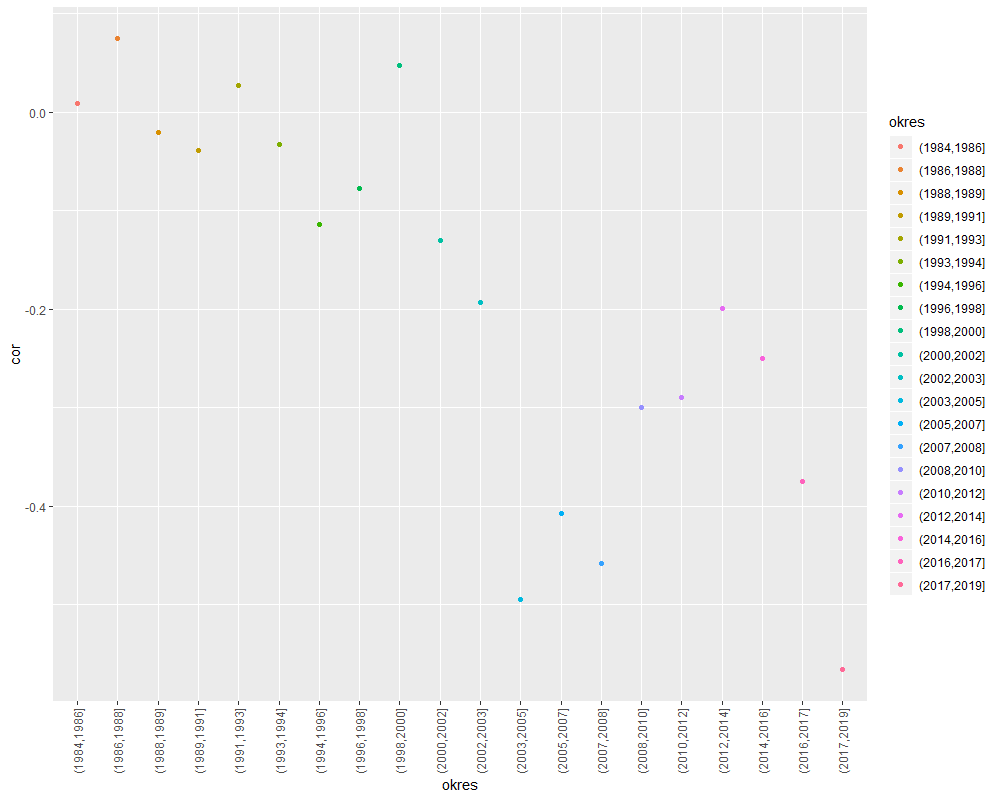
\includegraphics[width=\linewidth]{gold_USDPLN_korelacja_przedzialy.png}
\caption{Korelacja podziałem na 20 okresów}
\end{figure}

Oraz korelacja dla przedziałów $[i;06.2019]$, gdzie $i \in \{1984, \ldots, 06.2019\}$:
\newpage
\begin{figure}[ht!]
\centering
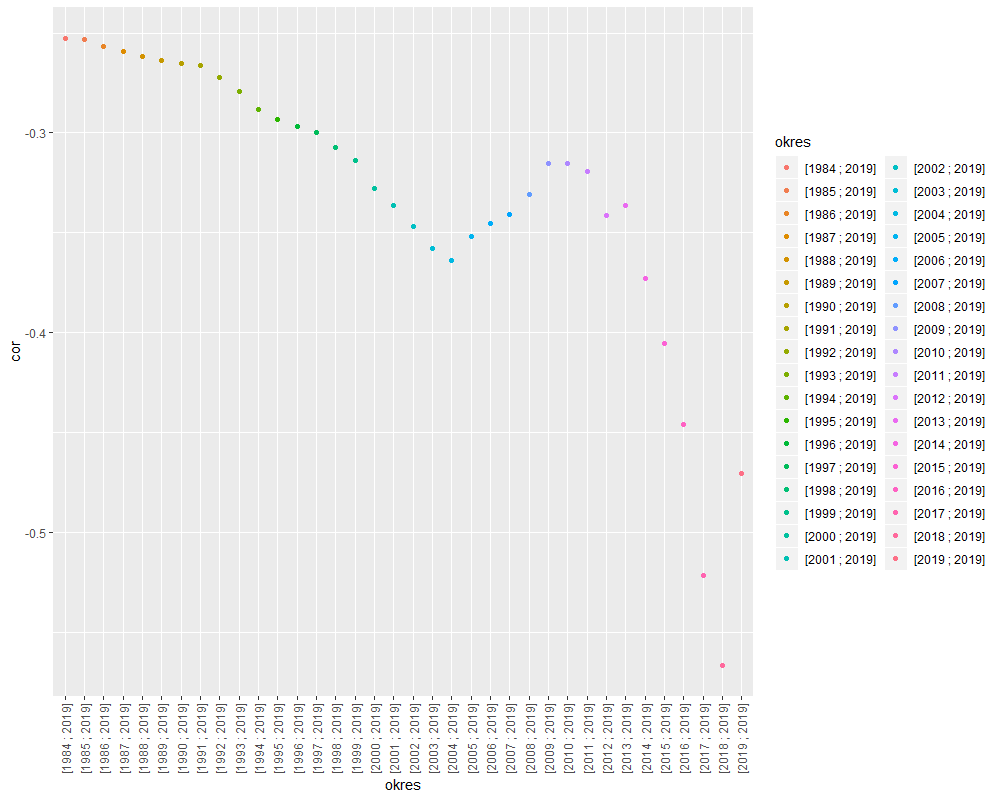
\includegraphics[width=\linewidth]{gold_USDPLN_korelacja_do_teraz.png}
\caption{Korelacja dla przedziałów}
\end{figure}

Na podstawie ww. analiz wybrano przedziały $2018 - 06.2019$ do estymacji dryfów rocznych, $2017 - 06.2019$ do estymacji zmienności rocznych oraz korelacji. W poniższej tabelce znajduje się zbiorcze podsumowanie wyestymowanych parametrów (dla zmienności i dryfu rocznego):

\begin{table}[h]
\begin{tabular}{|l|l|l|l|}
\hline
          & USDPLN & goldUSD & goldPLN \\ \hline
dryf      & 0.051  & 0.058   & 0.104   \\ \hline
zmienność & 0.089  & 0.098   & 0.095   \\ \hline
\end{tabular}
\end{table}

Korelacja pomiędzy $USDPL$N i $goldUSD$ została przyjęta na poziomie $-0.521$ co jest zgodne z sytuacją rynkową: wzrost wartości dolara powoduje spadek wartości złota. Korelacja pomiędzy $USDPLN$, a $goldPLN$ przyjęto na poziomie $0.382$.
\newline

Poniżej znajdują się kwantyle $1000$ wyestymowanych geometrycznych ruchów Browna dla poszczególnych kursów. Zostały one przedstawione na tle prawdziwych trajektorii:
\newpage
\begin{figure}[ht!]
\centering
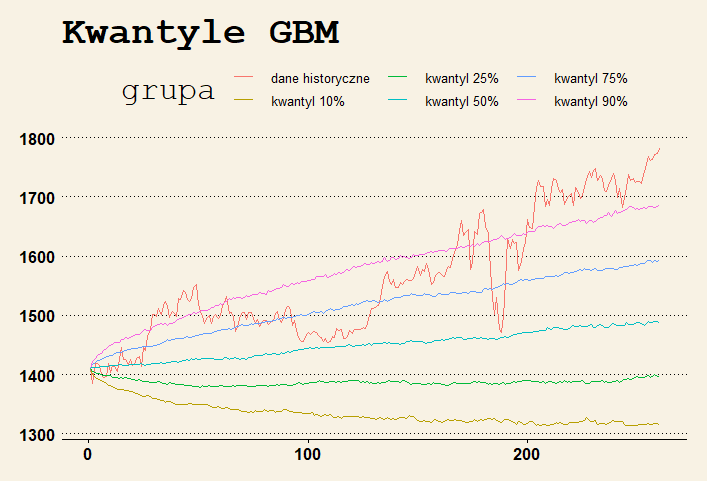
\includegraphics[width=\linewidth]{kwantyle_GBM_GOLD.png}
\caption{Kwantyle wyestymowanych trajektorii na tle historycznej trajektorii goldUSD}
\end{figure}
 
 Na powyższym wykresie widać, iż prawdziwa trajektoria oscyluje wokół kwantylu $0.9$. Nie jest to dobry rezultat, jednakże trzeba wziąć pod uwagę fakt, iż w tamtym okresie nastąpił duży wzrost złota w dolarach (o prawie $28\%$) - co jest sytuacją anomalną. 
 \newline
 Podobny rezultat będzie widoczny dla złota w złotówkach:
 
\newpage
\begin{figure}[ht!]
\centering
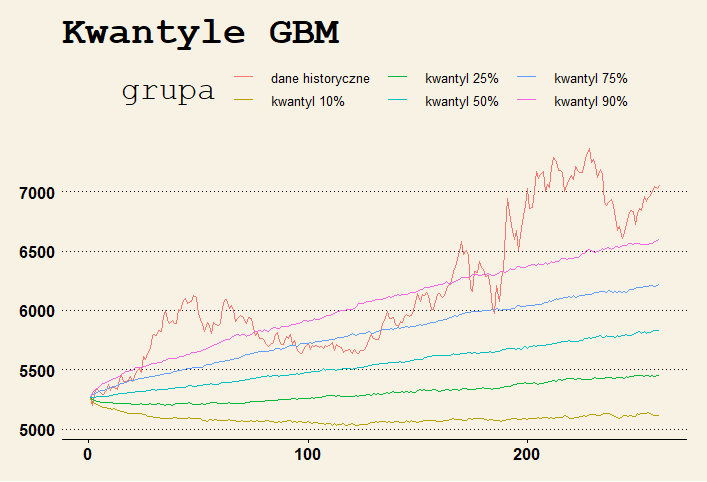
\includegraphics[width=\linewidth]{kwantyle_GBM_GOLDPLN.png}
\caption{Kwantyle wyestymowanych trajektorii na tle historycznej trajektorii goldPLN}
\end{figure}
\newpage

\newpage
\begin{figure}[ht!]
\centering
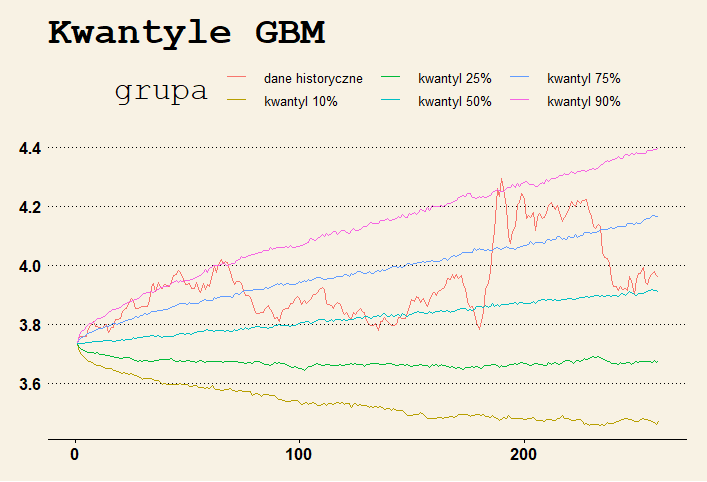
\includegraphics[width=\linewidth]{kwantyle_GBM_USDPLN.png}
\caption{Kwantyle wyestymowanych trajektorii na tle historycznej trajektorii USDPLN}
\end{figure}

Natomiast w tym przypadku kurs dolara oscyluje wokół mediany. Jest to sytuacja idealna. Intuicyjnie możemy założyć, iż nasze portfele, skonstruowane na trajektorii historycznej, będą zachowywały się najlepiej na podstawie tej trajektorii.

\newpage

\section{Portfele na wysymulowanych trajektoriach}
Naszym zadaniem jest sprawdzenie (przy pomocy symulacji) czy nasze strategie zabezpieczające dla
opcji quanto (\ref{Opcja quanto}). Strategia oparta na zbudowaniu portfela przez proces $USDPLN$ i $goldUSD$ (\ref{Wariant 1}) będzie oznaczana przez ,,wariant 1", natomiast strategia oparta na procesach $USDPLN$ i $goldPLN$ (\ref{Wariant 2}) będzie oznaczana przez ,,wariant 2". W rozdziale 2 udowodniono, że zabezpieczanie opcji quanto jest tożsame z zabezpieczaniem:
\begin{itemize}
    \item $\frac{100}{S_0}$ opcji call z ceną wykonania $KS_0$ na aktywo bazowe $S$, wypłacające ciągłą dywidendę $D=r-r_f+\rho_1 \sigma_1 \sigma_2$, gdzie $S$ to proces $goldUSD$, $r$ - krajowa stopa procentowa wolna od ryzyka, $r_f$ - zagraniczna stopa procentowa wolna od ryzyka, $\rho_1$ - korelacja pomiędzy procesami $goldUSD$ i $USDPLN$, $\sigma_1$ zmienność roczna procesu $goldUSD$, $\sigma_2$ zmienność roczna procesu $USDPLN$. - wariant 1
    \item $\frac{100 X_0}{Y_0}$ opcji call z ceną wykonania $K\frac{Y_0}{X_0}$ na aktywo bazowe $Z = \frac{Y}{X}$, wypłacające ciągłą dywidendę $D=r-r_f+\rho_2 \sigma_2 \sigma_3 - \sigma_2^2$, gdzie $Y$ to proces $goldPLN$, $X$ - proces $USDPLN$, $\rho_2$ - korelacja pomiędzy procesami $goldPLN$ i $USDPLN$, $\sigma_3$ zmienność roczna procesu $goldPLN$.
    W tym przypadku portfel ma postać $\Pi = W(Z,t) - \Delta Z$. Dryf roczny procesu $Z$ wynosi: $\mu_3 - \mu_2 + \sigma_3^2 - \rho_2 \sigma_3 \sigma_2$ ($\mu_2, \mu_3$ dryf roczny procesów $SUDPLN$ i $goldPLN$), natomiast zmienność roczna tego procesu to: $\sqrt{\sigma_3^2 + \sigma_2^2 - 2\rho_2 \sigma_3 \sigma_2}$. - wariant2
\end{itemize}
W obu przypadkach nasze portfele są w złotówkach.
\newline
Za stopę procentową wolną od ryzyka przyjęto procentowy stopę procentową z $10$-letnich obligacji państwowych, która była w $06.2019r.$. Przyjmujemy, że obie stopy mają stopę procentową równą $0.0212$ (stopa zagraniczna), ponieważ nasz portfel jest wrażliwy na zmiany stóp procentowych (pokażemy to w kolejnych rozdziałach). Przypomnijmy, że nasz portfel ma postać: 
$$\Pi = W(S,t) - \Delta_\$ S_\$ - \Delta S S_\$$$
Oba warianty mają takie same portfele, ponieważ pokazaliśmy, że te podejścia są równoważne (jeżeli spełnione są wszystkie warunki).
\\
Na podstawie parametrów wyestymowanych w rozdziale \ref{Kalibracja} parametry dla poszczególnych wariantów (parametry opcji oraz aktywów bazowych) prezentują się następująco:


\begin{table}[h]
\begin{tabular}{|l|l|l|}
\hline
          & wariant 1 & wariant 2 \\ \hline
dryf      & 0.051     & 0.059     \\ \hline
zmienność & 0.089     & 0.103     \\ \hline
korelacja & -0.521    & 0.382     \\ \hline
dywidenda & 0.00117   & 0.00100   \\ \hline
\end{tabular}
\end{table}

\newline
Oczywiście, jeżeli dywidenda jest wypłacana, to trzeba ją uwzględnić w kursie aktywa. W naszym przypadku uwzględniamy to w dryfie rocznym: przed wysymulowaniem trajektorii od dryfu rocznego odejmujemy dywidendę.
\newline
Będziemy symulować $1000$ trajektorii poszczególnych aktywów i sprawdzimy jak kształtuje się końcowy bilans ze względu na zmianę parametrów (stóp procentowych, ceny wykonania) oraz ze względu na częstotliwość rehedgowania.


\newpage

Poniżej zapiszemy algorytm zabezpieczania naszego portfela (niech $\delta$ oznacza ilość złota, potrzebną do zabezpieczenia opcji call na aktywie $S$, z ceną wykonania $KS_0$ i terminem zapadalności $1$, oraz $V_i^{S_i}$, to wartość opcji call w chwili $i$ na aktywie $S$ (złoto w dolarach) w chwili $i$, $S_{i}^\$$ to kurs dolara w chwili $i$):
\begin{enumerate}
    \item sprzedajemy $\frac{100}{S_0}V_0^{S_0}$  i uzyskujemy kapitał (w chwili 0), na początku mamy $0$ złota $(z)$ i $0$ dolarów $(d)$. Bilans w chwili $0$ wynosi $0$.
    \item w chwili $okres*i$ (okres w zależności od rehedgowania, $i * okres$ to jest dzień w którym się znajdujemy), podstawiamy $d_{old}=d$ i $z_{old}=z$ i wyznaczamy $\Delta=\frac{100}{S_0}\delta$. Mamy $z=\frac{\Delta}{S_{okres*i}^\$}$ i $d=\frac{-S_{okres*i}\Delta}{S_{okres*i}^\$}$.
    \item kapitał w chwili $i$, to kapitał (w chwili $i-1$) $-((d-d_{old})-(z-z_{old})*S_{okres*i})*S_{okres*i}^\$$
    \item liczymy kapitał na dzień $okres*(i+1)$. Wynosi on kapitał (w chwili i) $*e^{r\frac{dt okres}{n}} + z*S_{okres*i}*S_{okres*i}^\$*D*dt*okres$ 
    \item w chwili $i+1$, nasz $bilans = bilans - \frac{100}{S_{0}}V_{okres*(i+1)}^{S_{okres*(i+1)}} + z * S_{okres*i} *  S_{okres*i}^\$ + d * S_{okres*i}^\$ +  kapital$
    \item powtarzamy kroki 2-5, aż nie znajdziemy się w chwili $T$
\end{enumerate}

Na sam początek pokażemy, iż rezultaty dla obu podejść są takie same. Poprzez ,,okres" będziemy rozumieć liczbę dni po jakich rehedgujemy (np. gdy $okres=1$, to rehedgujemy codziennie). Poniżej znajduje się porównanie histogramów dla wariantu $1$ i $2$:
\newpage
\begin{figure}[ht!]
\centering
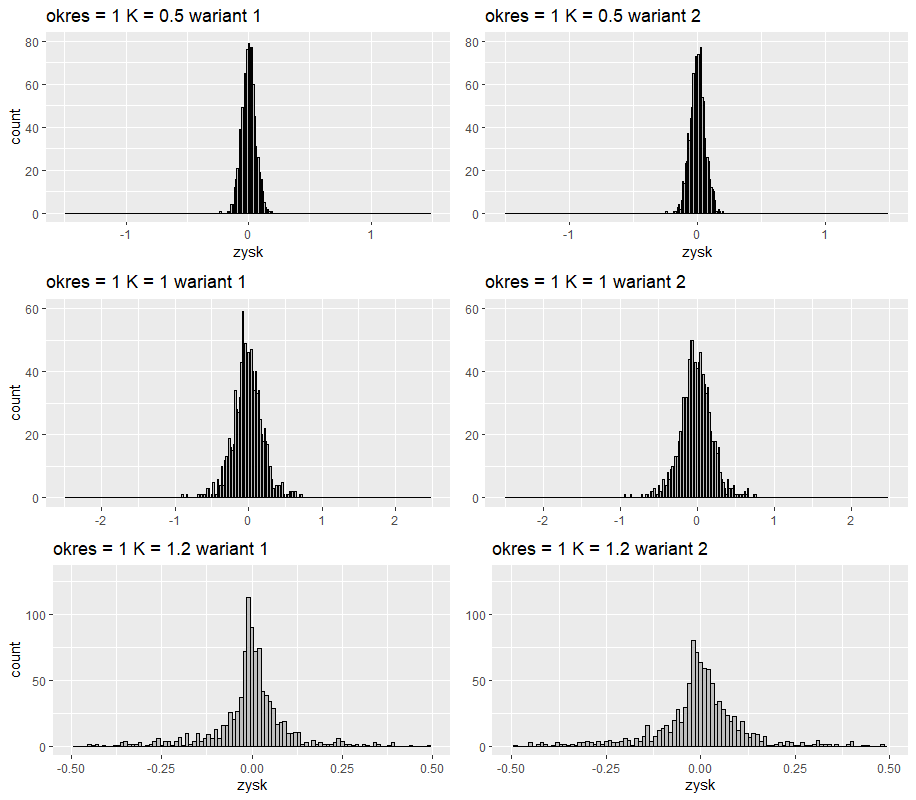
\includegraphics[width=\linewidth]{porownanie.png}
\caption{Porównanie bilansów z podziałem na warianty}
\end{figure}

Praktycznie nie ma różnic w poszczególnych wariantach (małe różnice występują z powodu za małej liczby symulacji, gdybyśmy ją zwiększyli, to histogramy by się pokryły). Z tego powodu w tym rozdziale będziemy rozważać wrażliwość bilansu (na zmiany parametrów) tylko dla jednego wariantu.
\newpage
\subsection{Zmiana częstotliwości rehedgowania}

\begin{figure}[ht!]
\centering
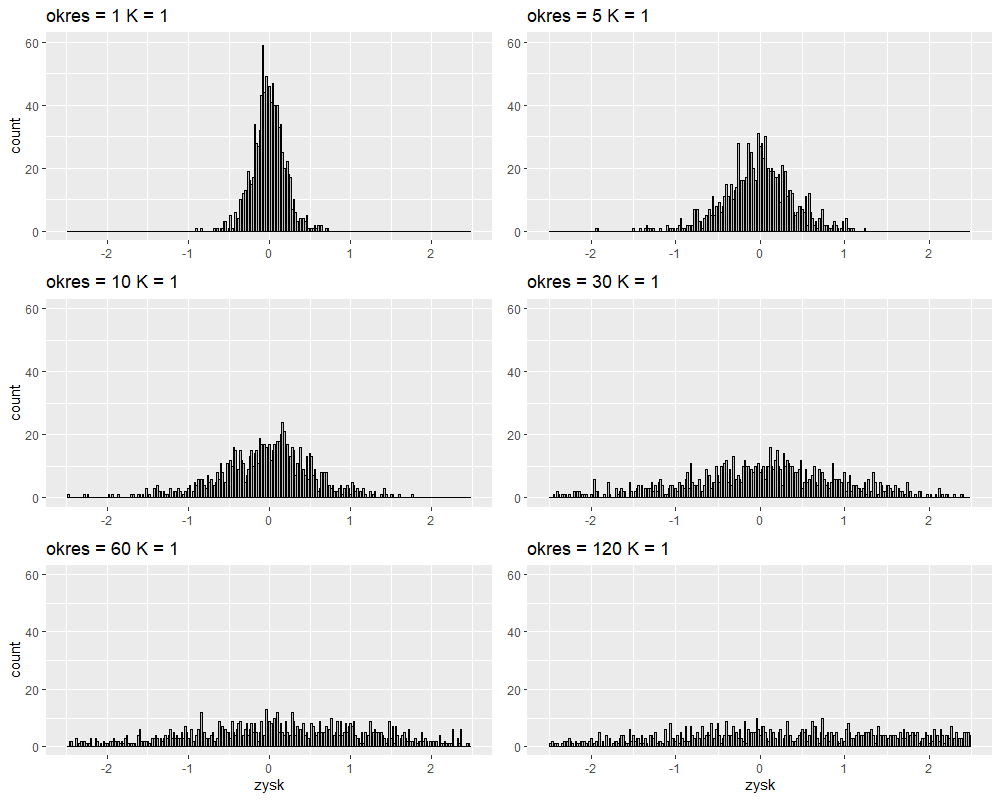
\includegraphics[width=\linewidth]{bilanse_gold_1.png}
\caption{Porównanie bilansów z różnym rehedgowaniem, K = 1}
\end{figure}

Gdy $K = 1$, to mamy sytuację podobną jak w projekcie $1szym$, gdzie ceną wykonania było $S_0$. Im rzadziej rehedgujemy, tym gorzej zabezpieczamy nasz portfel. Bierze się to głównie z początkowej niepewności dotyczącej tego czy nasza opcja się wykona lub nie (z tego powodu cena opcji i delta często się zmieniają) i im rzadziej rehedgujemy tym częściej ,,spóźniamy się" z odpowiednim zabezpieczeniem naszego portfela. Z powodu tego, że każda trajektoria się różni, to nasze zabezpieczenie staje się losowe (przy rzadkim rehedgowaniu). W ostatnim przypadku nasz zysk rozkłada się prawie równomiernie (z przewagą ujemnych wartości, ponieważ dryf roczny jest dodatni).

\newpage


\begin{figure}[ht!]
\centering
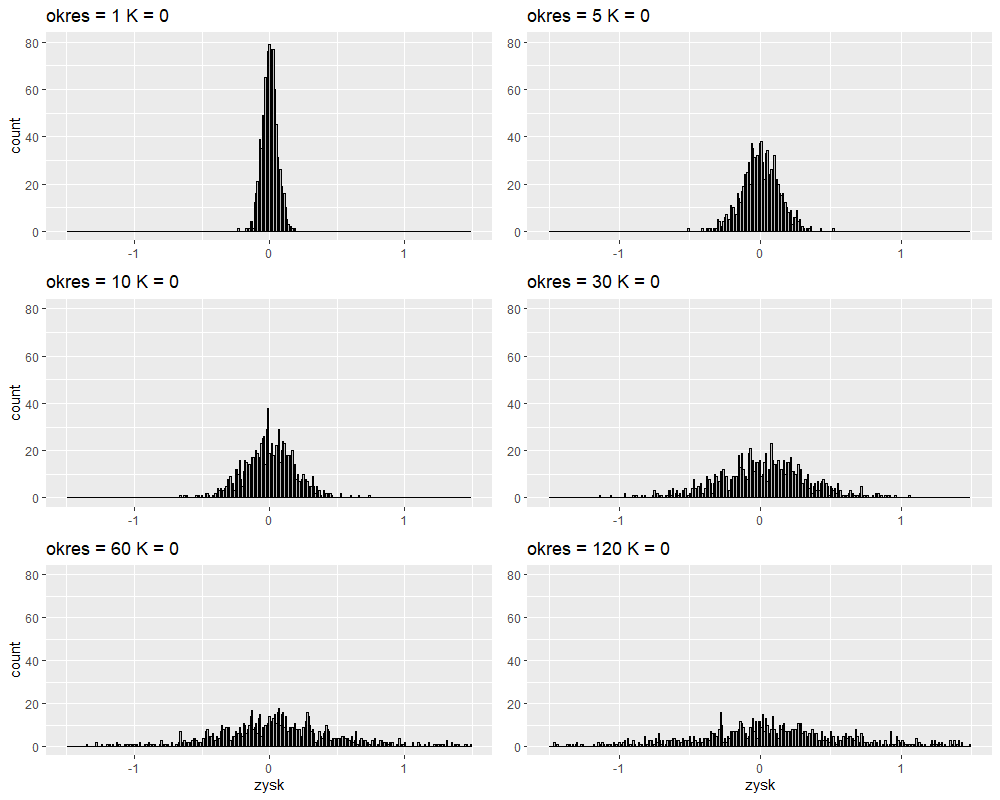
\includegraphics[width=\linewidth]{bilanse_gold_0.png}
\caption{Porównanie bilansów z różnym rehedgowaniem, K = 0}
\end{figure}

Tutaj następuje taka sytuacja, że nasza opcja zawsze się wykona. 
Opcja od samego początku jest warta praktycznie tyle samo co jej payoff (w chwili $i$). Dlatego nasza $\delta$ jest bliska $\frac{100}{S_0}$. Z tego powodu, że zmiany delty w czasie nie następują (są różnice tylko w z powodów numerycznych), to nasz bilans jest o wiele węższy od tego dla $K=1$. 

\newpage

Taka sama sytuacja następuje dla $K=0.5$ (występują różnice w tysięcznych) dlatego zostawimy to bez komentarza:

\begin{figure}[ht!]
\centering
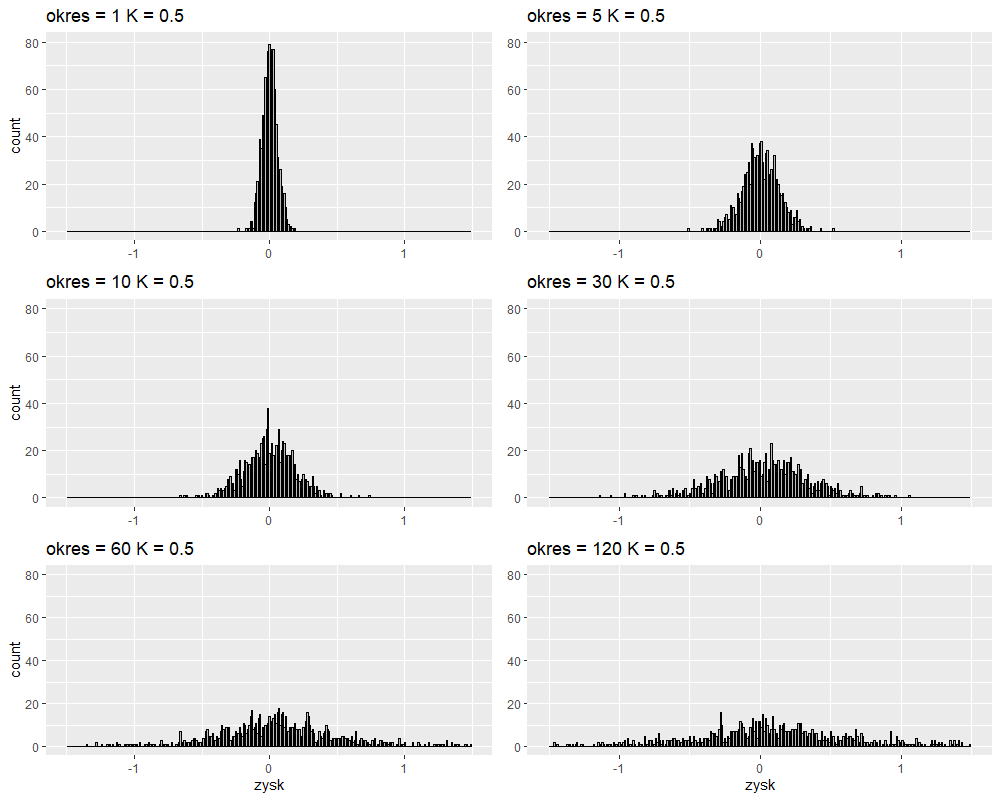
\includegraphics[width=\linewidth]{bilanse_gold_0.5.png}
\caption{Porównanie bilansów z różnym rehedgowaniem, K = 0.5}
\end{figure}


\newpage

\begin{figure}[ht!]
\centering
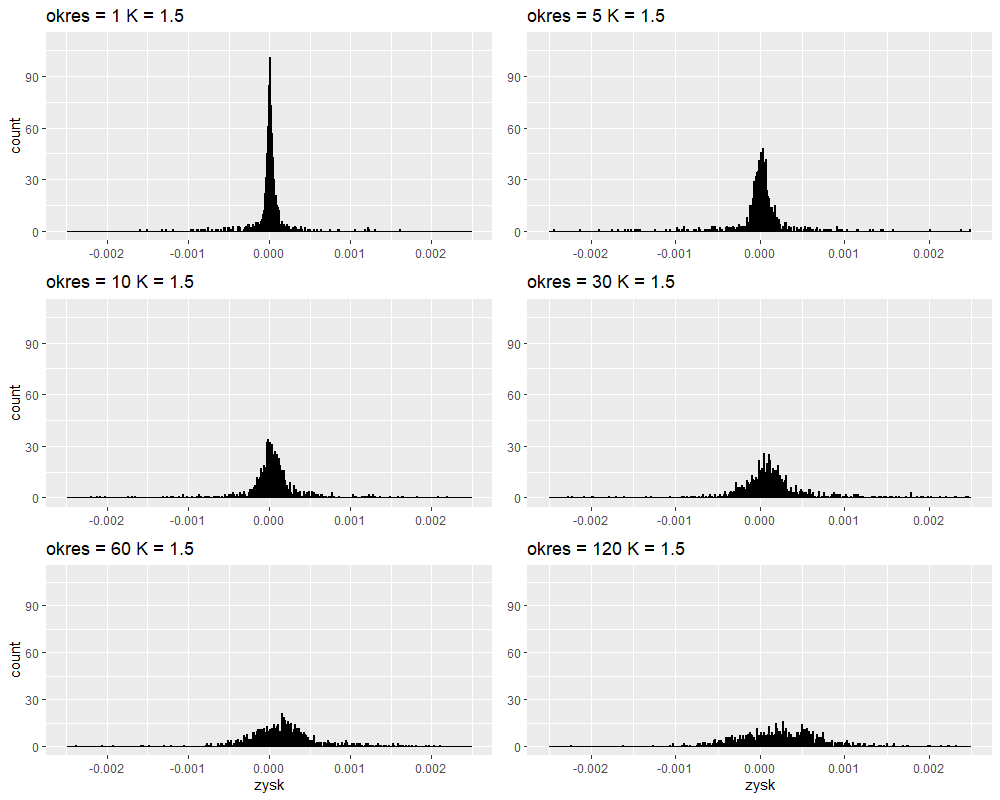
\includegraphics[width=\linewidth]{bilanse_gold_1.5.png}
\caption{Porównanie bilansów z różnym rehedgowaniem, K = 1.5}
\end{figure}

Dla $K=1.5$ p-stwo, że opcja się wykona jest równa bardzo blisko $0$ i z tego powodu wartość opcji też jest bliska $0$. Z tego powodu histogramy są bardzo zbliżone do $0$, ponieważ bardzo łatwo jest zabezpieczyć coś co jest bliskie $0$. Tutaj częstotliwość rehedgowania ma dużo mniejszy wpływ niż w poprzednich punktach. Ogólnie $2$ słupek się wyróżnia zapewne z błędów komputacyjnych (są tak małe wartości, że praktycznie za każdą z tych wartości moglibyśmy wpisać $0$).

\newpage

\begin{figure}[ht!]
\centering
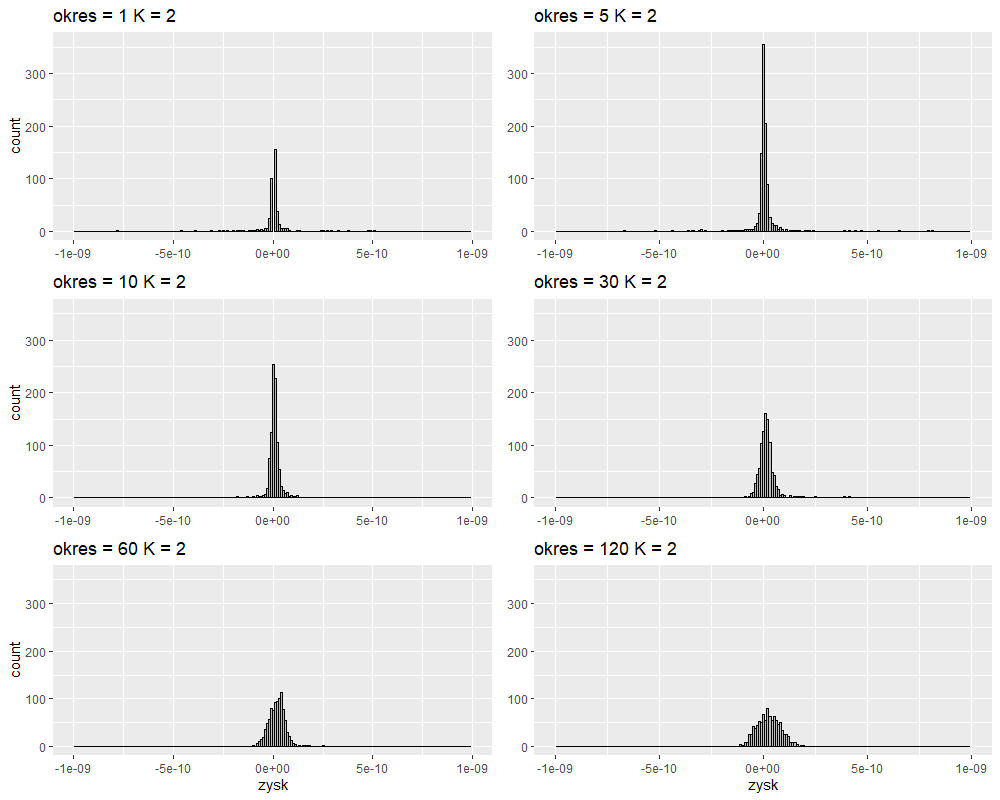
\includegraphics[width=\linewidth]{bilanse_gold_2.png}
\caption{Porównanie bilansów z różnym rehedgowaniem, K = 2}
\end{figure}

Tutaj następuje jeszcze mocniejsza sytuacja - mniejsza szansa na wykonanie opcji - wartość opcji jeszcze bliższa zeru - histogramy bardziej ,,zbite" wokół $0$.

\newline
W ogólności, biorąc pod uwagę powyższe rozważania, ,,najciekawsze" ceny wykonania są dla $K$ z przedziału $0.9$ i $1.3$, dlatego przyjrzymy się bliżej temu przedziałowi:
\newpage
\subsection{Zmiana ,,ciekawych" cen wykonania}

\begin{figure}[ht!]
\centering
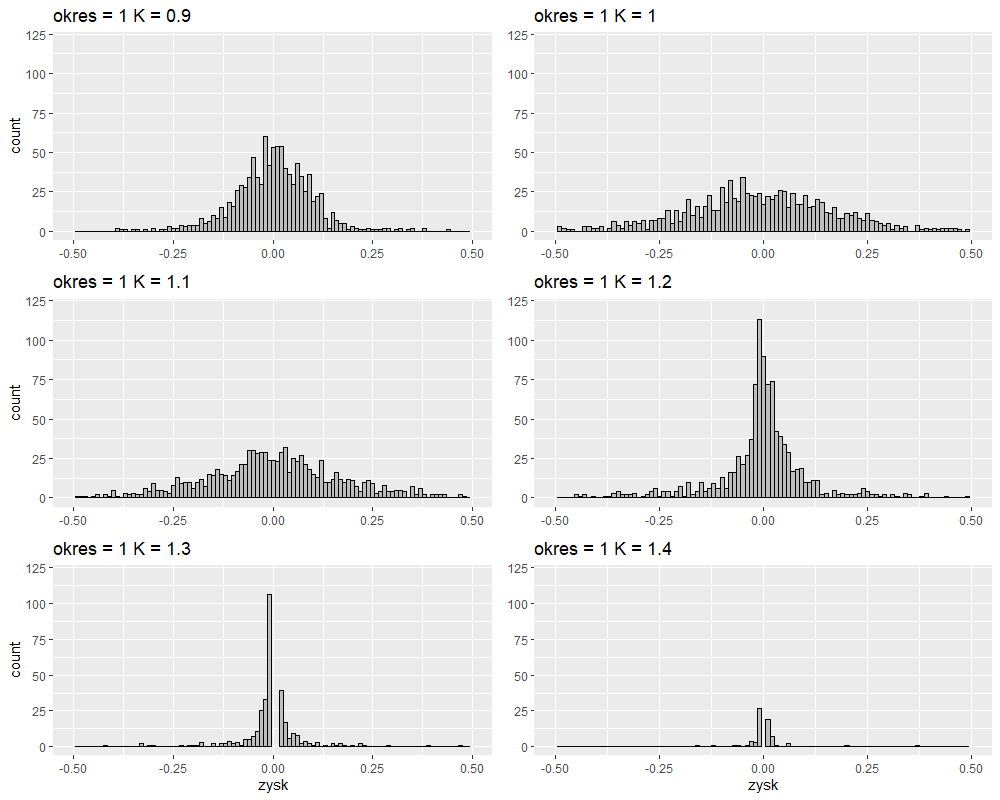
\includegraphics[width=\linewidth]{bilanse_gold_ciekawe_K.png}
\caption{Porównanie bilansów z różnym  $K \in \{0.9, 1, 1.1, 1.2, 1.3, 1.4\}$}
\end{figure}

Nasz wyestymowany dryf był bliski $5\%$, więc nasze przedziały są szersze dla K bliskich 1, ponieważ wtedy następują największe zmiany w wartości opcji. W ogólności, im jesteśmy bliżej $K=1$ (bardziej od strony dodatniej), to częściej musimy aktualizować $\delta$. Jak widzimy, praktycznie od $K=1.4$, nasz payoff jest na tyle mały, że nie następują duże zmiany w zmienności ceny opcji.


\newpage
\subsection{Zmiana parametrów $r$ i $r_f$}

Dobranie odpowiednich stóp procentowych ma istotny wpływ na uzyskiwane wyniki. W poniższych rozważaniach będziemy rozważać zmianę wartości $r - r_f$ (konkretne wartości $r$ i $r_f$ interesują nas mniej. Przypomnijmy, że w obu wariantach dywidenda $D$ zależała od różnicy $r - r_f$, a nie konkretnych wartości stóp. Wyniki dla $r=0.04, r_f=0.03$ były bardzo zbliżone do wyników dla $r=0.03, r_f=0.02$ - jeżeli nie będziemy przyjmować zdeprawowanych wartości stóp procentowych (bardzo wysokich), to wielkość tych parametrów nie ma istotnego wpływu na kształtowanie się końcowych bilansów). Ogólnie, model powinien być odporny na różnice w stopach procentowych. Jednakże wydaje nam się, że mamy poprawną implementację i widzimy, iż model jest wrażliwy na takie manipulacje. Prawdopodobnie wynika to z tego, że jeżeli stopa procentowa w USA jest większa od krajowej, to może istnieć możliwość arbitrażu (nie w sensie formalnym). Rozumiemy to przez to, że możemy skonstruować portfel, którego payoff będzie zawsze dodatni, ale z p-stwem zbliżonym do $0$.


\begin{figure}[ht!]
\centering
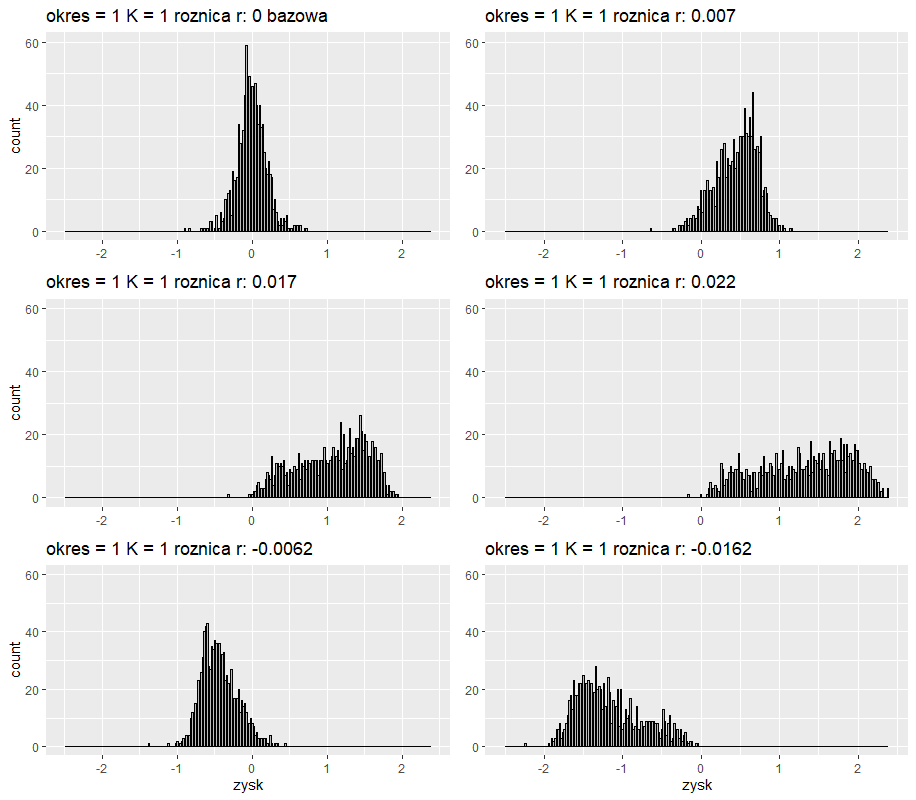
\includegraphics[width=\linewidth]{bilanse_gold_1_zmiana_r.png}
\caption{Porównanie bilansów z różnymi stopami procentowymi}
\end{figure}


\newpage

\section{Portfele na prawdziwych trajektoriach}

Tutaj zajmiemy się rozważaniem czy nasza konstrukcja portfela jest poprawna. W ogólności, pokazaliśmy wyżej, że wyniki dla obu wariantów są takie same, dlatego nie będziemy zajmować się analizą z podziałem na warianty. Ponadto, w rozdziale wyżej, pokazaliśmy, że nasza portfele są skonstruowane poprawnie - we Wszystkich przypadkach otrzymaliśmy histogramy bilansów skoncetrowane wokół wartości $0$, dlatego, w głównej mierze, wyniki mogą być zależne od poprawnego doboru parametrów. Poniżej znajduje się tabelka porównująca prawdziwe i wyestymowane wartości parametrów (w okresie $06.2019r.-06.2020r.)$:

\begin{table}[h]
\begin{tabular}{|l|l|l|l|l|l|l|}
\hline
          & estUSDPLN & USDPLN & estgoldUSD & goldUSD & estgoldPLN & goldPLN \\ \hline
dryf      & 0.051     & 0.056  & 0.058      & 0.267   & 0.104      & 0.322   \\ \hline
zmienność & 0.089     & 0.099  & 0.098      & 0.171   & 0.095      & 0.187   \\ \hline
\end{tabular}
\end{table}

Korelacja $goldUSD$ i $USDPLN$: $-0.521$ (wyestymowana), $-0.112$ (prawdziwa), natomiast pomiędzy $goldPLN$ i $USDPLN$: $0.382$ (wyestymowane), $0.367$ (prawdziwe).
\newline
W ogólności, najważniejsze jest poprawne dobranie zmienności. W każdym przypadku ją zaniżyliśmy, więc możemy mieć taką intuicję, że w praktycznie każdym przypadku będziemy mieć stratę (ponieważ opcja oparta na aktywie o większej zmienności jest droższa niż ta oparta na aktywie o mniejszej zmienności, ogólnie najlepszy hedging dokonuje się na ,,nudnym" aktywie, czyli takim, którego zachowanie jesteśmy w stanie przewidzieć).
\newpage
\subsection{Bilans w zależności od częstości rehedgowania}

\begin{figure}[ht!]
\centering
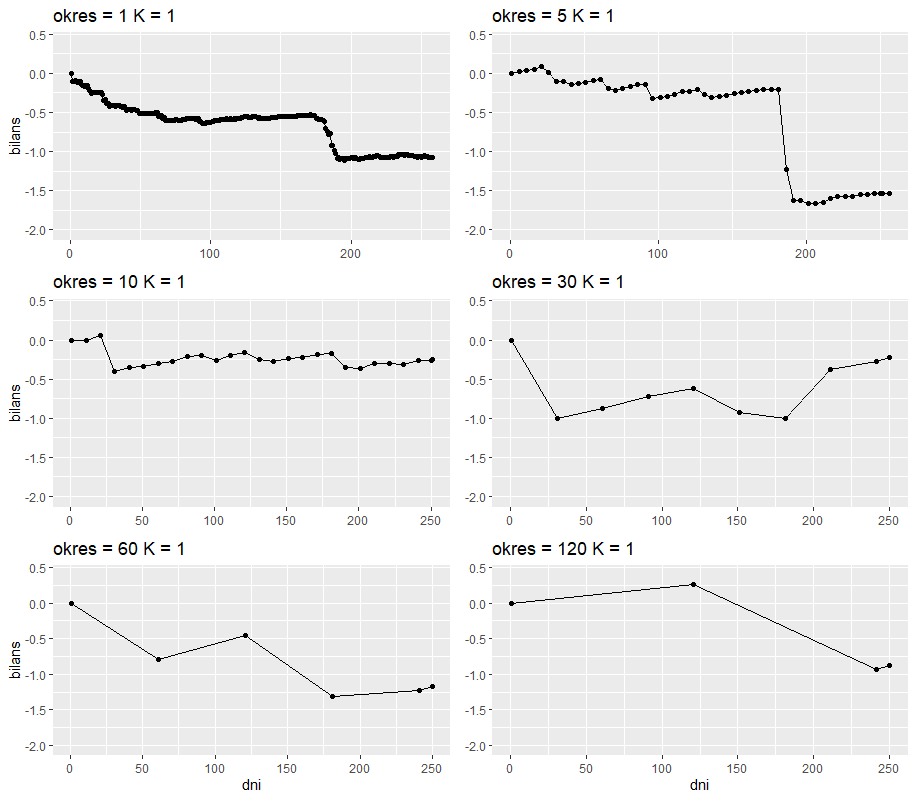
\includegraphics[width=\linewidth]{bilans_prawdziwa_trajektoria_gold_1_rowna_skala.png}
\caption{Porównanie bilansów w zależności od częstości rehedgowania, $K=1$}
\end{figure}

W ogólności, dokonamy tylko jednej analizy częstości rehedgowania, ponieważ dla pozostałych $K$ wyniki będą podobne. W tym przypadku widzimy, iż zawsze tracimy (m.in z powodu niedoszacowania zmienności rocznej). Jednakże ta strata jest mała i można by ją zniwelować poprzez dodatkowe zabezpieczenie (np. poprzez procentowe zwiększenie początkowej wartości opcji). Ponadto widzimy, iż dla częstość rehedgowania nie ma dużego wpływu na wielkość straty. Jednakże jest to sytuacja losowa i strata mogłaby być dużo większa (na symulacjach pokazaliśmy, że im częściej rehedgujemy, tym bilans się rozkłada bardziej jednostajnie. Oczywiście taka sytuacja zachodzi dla odpowiednich $K$ - nie za dużych i nie za małych).

\newpage
\subsection{Bilans w zależności od zmiany ,,nieciekawych" $K$}

\begin{figure}[ht!]
\centering
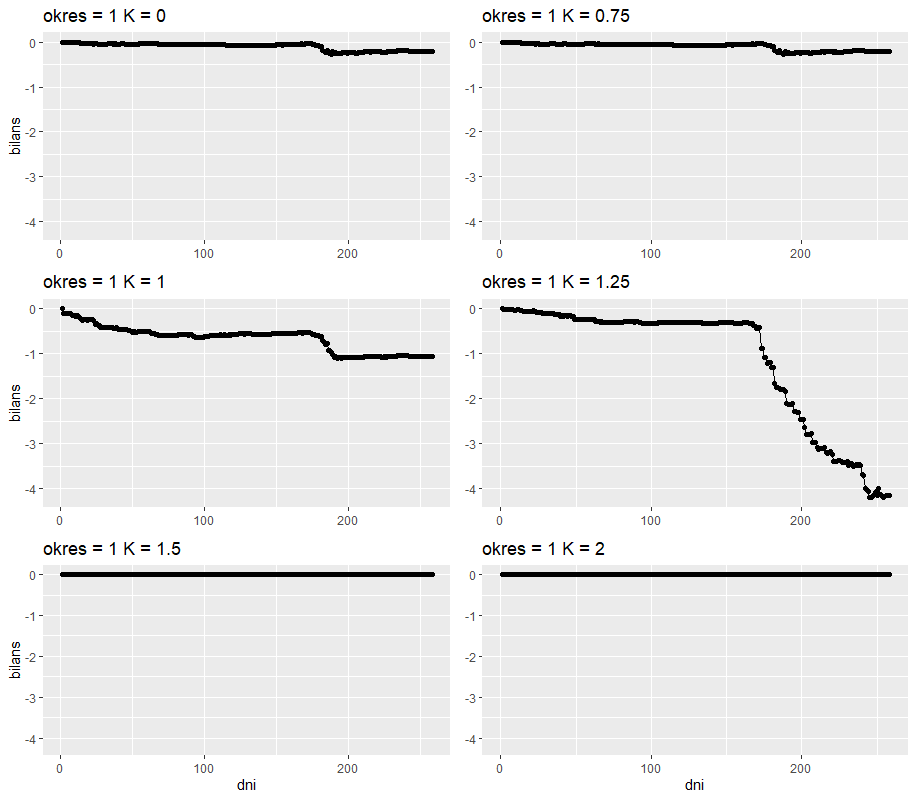
\includegraphics[width=\linewidth]{bilans_prawdziwa_trajektoria_gold_zmiana_K_nieciekawe_rowna_skala.png}
\caption{Porównanie bilansów w zależności od zmiany $K$}
\end{figure}

Cena złota $30.06.2019r.$ wynosiła $1409$ dolarów, natomiast $30.06.2020r.$ wynosiła $1770$ dolarów. W ogólności bilanse są bardzo bliskie $0$, gdy opcja prawie na pewno się nie wykona lub prawie na pewno się wykona. Dopiero ciekawsze sytuacje się pojawiają dla $K \in \{0.9, 1.3\}$, czyli dla takich, które na samym początku nie mają p-stwa wykonania się, które jest zbliżone do $1$ (lub $0$), a zostaną wykonane w terminie zapadalności (przypomnijmy, że prawdziwy dryf był w okolicach $26\%$). Poniżej zobaczymy jak bilans się kształtuje dla ,,ciekawszych" $K$:
\newpage

\subsection{Bilans w zależności od zmiany ,,ciekawych" $K$}

\begin{figure}[ht!]
\centering
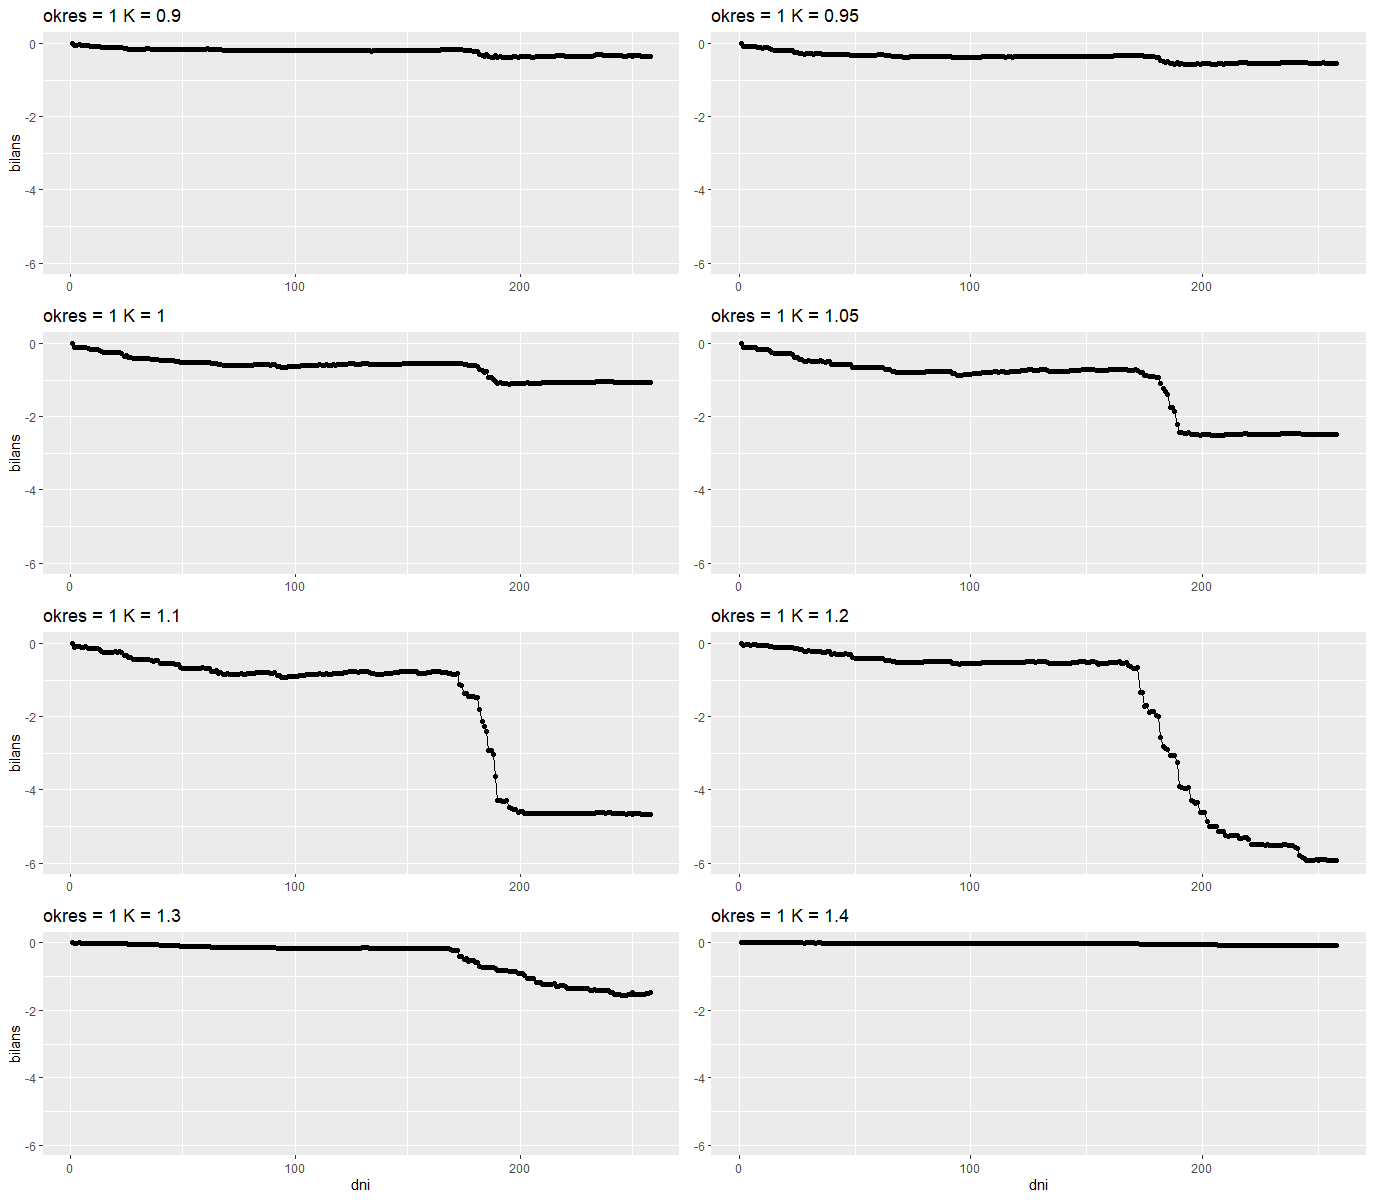
\includegraphics[width=\linewidth]{bilans_prawdziwa_trajektoria_gold_zmiana_K_ciekawe_rowna_skala.png}
\caption{Porównanie bilansów w zależności od zmiany $K$}
\end{figure}

Jak widzimy, ponownie mamy małą stratę (którą można łatwo skompensować za pomocą zabezpieczenia), która wynika z niedoszacowania zmienności. Dla $K=1.3$ bilans staje się ujemny, gdy opcja zaczyna być coś warta (czyli gdy cena złota mocno wzrasta, do okolic $1600$ dolarów). W ogólności największy spadek się pojawia dla okresu $18-24.02.2020r.$, wtedy następuje wzrost wartości złota o prawie $100$ dolarów. Ten nagły wzrost wartości złota wynika m.in. z rosnącego niepokoju społecznego, wynikającego z rozprzestrzeniania się wirusa COVID-19. Wtedy pojawiały się pierwsze większe ogniska poza Chinami. Powszechnie istnieje przekonania, że złoto jest uniwersalną metodą płatności, dlatego idealnie się nadaje na sytuacje kryzysowe. Wtedy więcej ludzi dokonało zakupu złota, co mogło spowodować nagły wzrost wartości złota. Gdyby takowa sytuacja nie nastąpiła, to nasz portfel przyniósłby o wiele mniejsze straty. 
\newpage
\subsection{Bilans w zależności od zmiany stóp procentowych}

\begin{figure}[ht!]
\centering
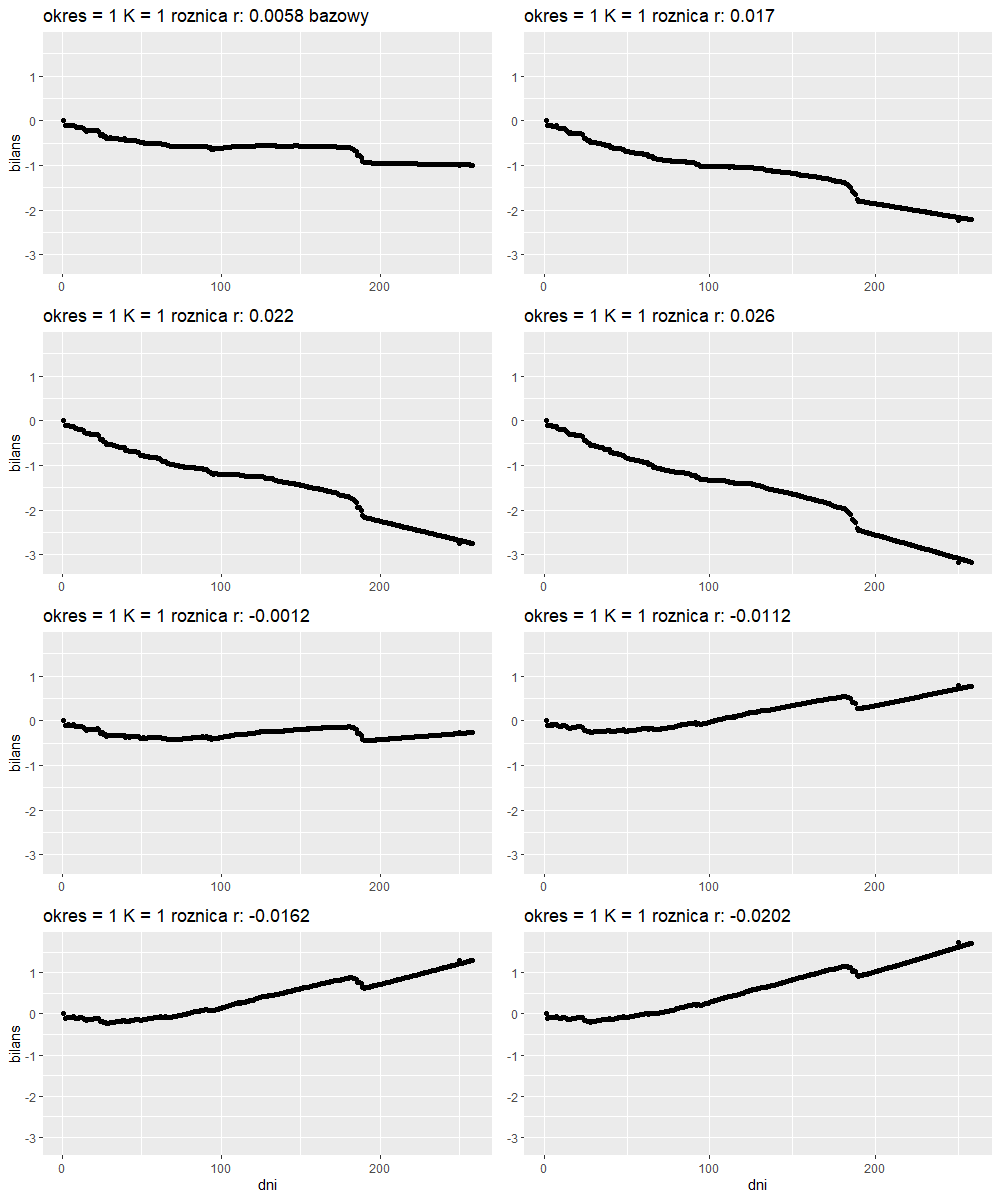
\includegraphics[width=\linewidth]{bilans_prawdziwa_trajektoria_gold_zmiana_r_rowna_skala.png}
\caption{Porównanie bilansów w zależności od zmiany stóp procentowych}
\end{figure}

Tutaj następuje taka sytuacja jak na wysymulowanych trajektoriach.



\newpage

\section{Inne opcje na złoto}

Rozważamy opcję pozwalającą na zakup w chwili T złota po cenie $S(0)X(0)$ PLN, gdzie
\begin{itemize}
    \item $S(t)$ - cena złota w dolarach w chwili t
    \item $X(t)$ - kurs wymiany dolara na złotówki w chwili t
\end{itemize}
Przeanalizujemy zachowanie takiej opcji z punktu widzenia inwestora w Polsce i w USA. 
Dla inwestora w Polsce payoff takiej opcji wynosi 
\[
\text{Payoff} = \Big(S(T)X(T) - S(0)X(0)\Big)^+
\]
gdyż inwestor po wykonaniu opcji w chwili $T$ i zakupie złota ze cenę $S(0)X(0)$ sprzedaje je za $S(T)$ dolarów - musi więc przekonwertować je jeszcze na złotówki po kursie $X(T)$. 

Stosując podstawienie $Y(t) = S(t)X(t)$ jest to payoff zwykłej opcji call na cenę $S(0)X(0)$. Zakładamy, że
\[
X(t) = X(0)e^{\big(\mu_X - \frac {\sigma_X^2} 2\big) t + \sigma_X B(t)} \hspace{5mm} S(t) = S(0)e^{\big(\mu_S - \frac {\sigma_S^2} 2\big) t + \sigma_S B'(t)} 
\]
gdzie $B$, $B'$ są ruchami Browna o korelacji $\rho$. Wtedy oznaczając \[
\sigma_Y = \sqrt{\sigma_X^2 + \sigma_S^2 + 2\rho \sigma_X \sigma_S} \hspace{5mm} \mu_Y = \mu_X + \mu_S + 2\rho \sigma_X \sigma_Y
\] 

oraz korzystając z faktu, że dla ruchów Browna $B$, $B'$ mamy, że $\sigma_X B(t) + \sigma_S B'(t) = \sigma_Y W(t)$, gdzie $W$ też jest ruchem Browna, otrzymujemy
\[
Y(t) = Y(0)e^{\big(\mu_Y - \frac {\sigma_Y^2} 2\big) + \sigma_Y W(t)}
\]
Czyli $Y(t)$ również jest geometrycznym ruchem Browna. Stąd wycenę takiej opcji możemy wykonywać przy użyciu znanych wzorów dla opcji call wyprowadzonych z modelu Blacka-Scholesa. 

W porównaniu z opcjami quanto podstawowa różnica tutaj jest taka, że payoff tej opcji jest wrażliwy na zmianę kursu dolara. Niezależnie od wzrostu ceny złota payoff może pozostać zerowy, jeśli kurs dolara znacząco spadnie.

Z punktu widzenia inwestora w USA sytuacja ma się nieco inaczej; w tym wypadku inwestor przed wykonaniem opcji musi zamienić dolary na PLN, więc w swojej walucie musi za to złoto zapłacić $\frac {S(0)X(0)} {X(T)}$. Wtedy dla niego payoff wynosi 
\[
\text{Payoff} = \Big( S(T) - \frac {S(0)X(0)} {X(T)}\Big)^+ = S(0) \Big( \frac {S(T)} {S(0)} - \frac {X(0)} {X(T)} \Big)^+
\]

Podstawiając $Z(t) = \frac 1 {X(t)}$ jest to wzór na  payoff $S(0)$ sztuk opcji exchange, czyli opcji pozwalającej na wymianę jednego dobra na drugie - konkretnie złotówek na złoto. 

W porównaniu z poprzednią sytuacją jest tu podstawowa różnica - inwestor może zarobić nawet wtedy, gdy cena złota spadnie, jeśli tylko kurs PLN spadnie bardziej.

Ponownie możemy zaobserwować, że jeśli 
\[
X(t) = X(0)e^{\big( \mu - \frac {\sigma_X^2} 2\big) t + \sigma_X B(t)}
\] 
to
\[
Z(t) = Z(0) e^{\big((-\mu_X + \sigma_X^2) - \frac {\sigma_X^2} 2\big) t + \sigma_X(-B(t))}
\]
Więc korzystając tym razem z faktu, że $-B(t)$ jest ruchem Browna otrzymujemy, że $Z(t)$ to też geometryczny ruch Browna (z dryfem $\mu_Z = \mu_X + \sigma_X^2$). Przy wycenie takiej opcji można więc skorzystać ze znanych wzorów na cenę opcji exchange. 
\end{document}
